\documentclass{article}
\usepackage[a4paper,left=3cm, right=3cm, top=2cm, bottom=2cm]{geometry}
\usepackage{amsmath}
\usepackage{graphicx}
\usepackage{caption}
\usepackage{setspace}
\usepackage{xcolor}
\usepackage{titlesec}
\usepackage{amssymb}
\usepackage{tcolorbox}
\usepackage{wrapfig}
\usepackage{amsthm} % For proofs

\graphicspath{{graph/}}
\title{11.5 Alternating Series}
\date{}
\author{}
\setstretch{1.3} 

% \subsection* 형식 지정 (번호 없음)
\titleformat{name=\section, numberless}
  {\normalfont\large\bfseries\color{blue}}
  {}
  {0pt}
  {}
\geometry{a4paper, margin=1in}

% 증명 환경 스타일
\newtheoremstyle{mystyle}% name
  {}% Space above
  {}% Space below
  {\itshape}% Body font
  {}% Indent amount
  {\bfseries}% Theorem head font
  {.}% Punctuation after theorem head
  {.5em}% Space after theorem head
  {}% Theorem head spec (can be left empty, meaning `normal')
\theoremstyle{mystyle}

\begin{document}
\maketitle

The convergence tests that we have looked at so far apply only to series with positive terms. In this section and the next we learn how to deal with series whose terms are not necessarily positive.

\section*{Alternating Series}
An \textbf{alternating series} is a series whose terms are alternately positive and negative. Here are two examples:
\[ 1 - \frac{1}{2} + \frac{1}{3} - \frac{1}{4} + \frac{1}{5} - \cdots = \sum_{n=1}^{\infty} (-1)^{n-1} \frac{1}{n} \]
\[ -\frac{1}{2} + \frac{2}{3} - \frac{3}{4} + \frac{4}{5} - \frac{5}{6} + \cdots = \sum_{n=1}^{\infty} (-1)^{n} \frac{n}{n+1} \]
We see from these examples that the nth term of an alternating series is of the form \( a_n = (-1)^{n-1}b_n \) or \( a_n = (-1)^n b_n \), where \(b_n\) is a positive number.

\begin{tcolorbox}[
    colback=white,
    colframe=orange!80!white,
    title=The Alternating Series Test,
    boxrule=0.5mm,
    arc=3mm
    ]
    If the alternating series
    \[ \sum_{n=1}^{\infty} (-1)^{n-1}b_n = b_1 - b_2 + b_3 - b_4 + \cdots \quad (b_n > 0) \]
    satisfies
    \begin{itemize}
        \item[(i)] \( b_{n+1} \le b_n \) for all \(n\)
        \item[(ii)] \( \lim_{n\to\infty} b_n = 0 \)
    \end{itemize}
    then the series is convergent.
\end{tcolorbox}

\begin{figure}[htbp]
  \centering
  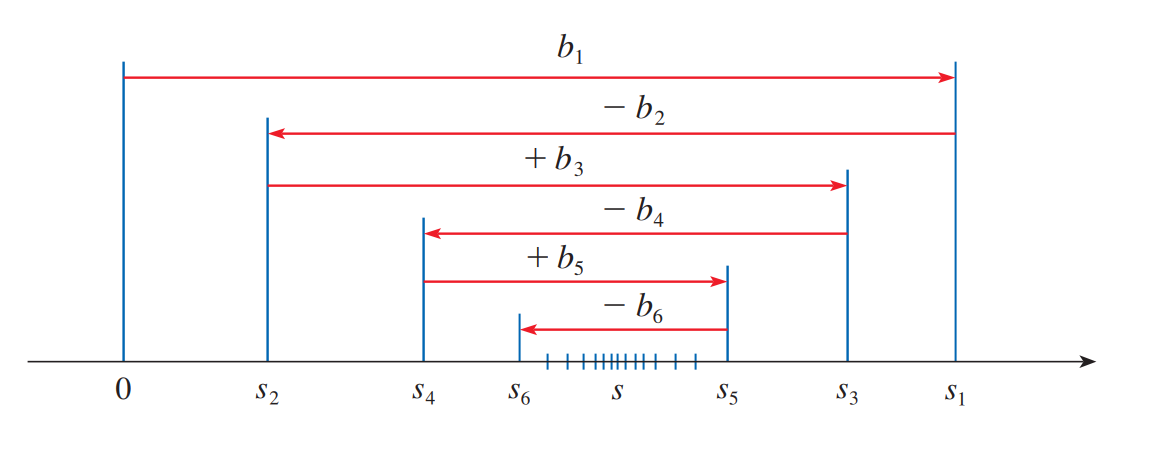
\includegraphics[width=0.6\textwidth]{graph76.png}
\end{figure}

\begin{proof}
[Proof]
First we consider the even partial sums:
\[ s_2 = b_1 - b_2 \ge 0 \]
\[ s_4 = s_2 + (b_3 - b_4) \ge s_2 \]
In general, \( s_{2n} = s_{2n-2} + (b_{2n-1} - b_{2n}) \). Since \(b_{2n} \le b_{2n-1}\), we have \(s_{2n} \ge s_{2n-2}\).
Thus, the sequence of even partial sums is increasing: \( s_2 \le s_4 \le s_6 \le \cdots \le s_{2n} \le \cdots \).
Also, we can write \( s_{2n} = b_1 - (b_2 - b_3) - (b_4 - b_5) - \cdots - (b_{2n-2} - b_{2n-1}) - b_{2n} \).
Every term in parentheses is positive, so \( s_{2n} \le b_1 \) for all \(n\).
Therefore, the sequence \(\{s_{2n}\}\) of even partial sums is increasing and bounded above. It is therefore convergent by the Monotonic Sequence Theorem. Let's call its limit \(s\), so
\[ \lim_{n\to\infty} s_{2n} = s \]
Now we compute the limit of the odd partial sums:
\[ \lim_{n\to\infty} s_{2n+1} = \lim_{n\to\infty} (s_{2n} + b_{2n+1}) = \lim_{n\to\infty} s_{2n} + \lim_{n\to\infty} b_{2n+1} = s + 0 = s \]
Since both the even and odd partial sums converge to \(s\), the sequence \(\{s_n\}\) converges to \(s\).
\end{proof}

\subsection*{EXAMPLE 1}
The alternating harmonic series
\[ 1 - \frac{1}{2} + \frac{1}{3} - \frac{1}{4} + \cdots = \sum_{n=1}^{\infty} \frac{(-1)^{n-1}}{n} \]
\textbf{SOLUTION:}
We have \(b_n = 1/n\).
\begin{itemize}
    \item[(i)] \(b_{n+1} = \dfrac{1}{n+1} < \dfrac{1}{n} = b_n\) because \(n+1 > n\). So \(\{b_n\}\) is decreasing.
    \item[(ii)] \( \lim_{n\to\infty} b_n = \lim_{n\to\infty} \dfrac{1}{n} = 0 \).
\end{itemize}
Both conditions of the Alternating Series Test are satisfied, so the series is \textbf{convergent}.

\subsection*{EXAMPLE 2}
Test the series \( \sum_{n=1}^{\infty} (-1)^n \dfrac{3n}{4n-1} \) for convergence or divergence.\\
\textbf{SOLUTION:}
Here \(b_n = \dfrac{3n}{4n-1}\). We check condition (ii):
\[ \lim_{n\to\infty} b_n = \lim_{n\to\infty} \dfrac{3n}{4n-1} = \lim_{n\to\infty} \dfrac{3}{4 - 1/n} = \dfrac{3}{4} \]
Since \( \lim_{n\to\infty} b_n = 3/4 \neq 0 \), condition (ii) is not satisfied. Instead, we look at the limit of the nth term of the series:
\[ \lim_{n\to\infty} a_n = \lim_{n\to\infty} (-1)^n \dfrac{3n}{4n-1} \]
This limit does not exist. So the series \textbf{diverges} by the Test for Divergence.

\subsection*{EXAMPLE 3}
Test the series \( \sum_{n=1}^{\infty} (-1)^{n+1} \dfrac{n^2}{n^3+1} \) for convergence.\\
\textbf{SOLUTION:}
Here \(b_n = \dfrac{n^2}{n^3+1}\).
\[ \lim_{n\to\infty} b_n = \lim_{n\to\infty} \dfrac{n^2}{n^3+1} = \lim_{n\to\infty} \dfrac{1/n}{1+1/n^3} = 0 \]
So condition (ii) is satisfied. To check condition (i), we consider the function \(f(x) = \dfrac{x^2}{x^3+1}\).
\[ f'(x) = \dfrac{(x^3+1)(2x) - x^2(3x^2)}{(x^3+1)^2} = \dfrac{2x^4+2x-3x^4}{(x^3+1)^2} = \dfrac{x(2-x^3)}{(x^3+1)^2} \]
Since we are considering positive \(x\), \(f'(x) < 0\) if \(2-x^3 < 0\), that is, \(x > \sqrt[3]{2}\).
So \(f\) is decreasing on \((\sqrt[3]{2}, \infty)\). This means that \(b_{n+1} < b_n\) when \(n \ge 2\). The conditions of the Alternating Series Test are satisfied (for \(n \ge 2\)), so the series is \textbf{convergent}.

\section*{Estimating Sums}
For a convergent alternating series, we can estimate the sum by a partial sum \(s_n\). The error involved is given by the following theorem.

\begin{tcolorbox}[
    colback=white,
    colframe=orange!80!white,
    title=Alternating Series Estimation Theorem,
    boxrule=0.5mm,
    arc=3mm
    ]
    If \(s = \sum (-1)^{n-1} b_n\) is the sum of a convergent alternating series with \(0 \le b_{n+1} \le b_n\), then
    \[ |R_n| = |s - s_n| \le b_{n+1} \]
    In words: the size of the error is at most the absolute value of the first neglected term.
\end{tcolorbox}

\begin{proof}
[Proof]
From the proof of the Alternating Series Test, we know that the true sum \(s\) lies between any two consecutive partial sums \(s_n\) and \(s_{n+1}\). It follows that
\[ |s - s_n| \le |s_{n+1} - s_n| \]
And since \( |s_{n+1} - s_n| = |a_{n+1}| = b_{n+1} \), we have
\[ |s - s_n| \le b_{n+1} \]
\end{proof}

\subsection*{EXAMPLE 4}
Find the sum of the series \( \sum_{n=0}^{\infty} \dfrac{(-1)^n}{n!} \) correct to three decimal places.\\
\textbf{SOLUTION:}
We first observe that the series is convergent by the Alternating Series Test because
\begin{itemize}
    \item[(i)] \(b_{n+1} = \dfrac{1}{(n+1)!} = \dfrac{1}{(n+1)n!} < \dfrac{1}{n!} = b_n\)
    \item[(ii)] \(0 \le \dfrac{1}{n!} \le \dfrac{1}{n} \to 0\), so \( \lim_{n\to\infty} \dfrac{1}{n!} = 0 \)
\end{itemize}
To get a sum correct to three decimal places, we need the error to be less than 0.0005. The error is given by \(|s - s_n| \le b_{n+1}\).
We calculate the first few terms:
\begin{align*}
    b_0 &= 1/0! = 1 \\
    b_1 &= 1/1! = 1 \\
    b_2 &= 1/2! = 0.5 \\
    b_3 &= 1/3! = 1/6 \approx 0.166667 \\
    b_4 &= 1/4! = 1/24 \approx 0.041667 \\
    b_5 &= 1/5! = 1/120 \approx 0.008333 \\
    b_6 &= 1/6! = 1/720 \approx 0.001389 \\
    b_7 &= 1/7! = 1/5040 \approx 0.000198
\end{align*}
Since \(b_7 < 0.0005\), we can stop at \(n=6\). The partial sum \(s_6\) is:
\[ s_6 = \frac{1}{0!} - \frac{1}{1!} + \frac{1}{2!} - \frac{1}{3!} + \frac{1}{4!} - \frac{1}{5!} + \frac{1}{6!} = 1 - 1 + 0.5 - 0.166667 + 0.041667 - 0.008333 + 0.001389 \approx 0.368056 \]
Rounding to three decimal places, we have \(s \approx 0.368\).

\section*{Absolute and Conditional Convergence}
Given any series \( \sum a_n \), we can consider the corresponding series of absolute values \( \sum |a_n| \).

\begin{tcolorbox}[
    colback=white,
    colframe=orange!80!white,
    title=Definition of Absolute and Conditional Convergence,
    boxrule=0.5mm,
    arc=3mm
    ]
    A series \( \sum a_n \) is called \textbf{absolutely convergent} if the series of absolute values \( \sum |a_n| \) is convergent.
    
    \vspace{1em}
    
    A series \( \sum a_n \) is called \textbf{conditionally convergent} if it is convergent but not absolutely convergent.
\end{tcolorbox}

\subsection*{EXAMPLE 5}
Determine whether the following series are absolutely convergent, conditionally convergent, or divergent.
\( \sum_{n=1}^{\infty} \dfrac{(-1)^{n-1}}{n^2} \) \quad \\
\textbf{SOLUTION:}
The series of absolute values is \( \sum_{n=1}^{\infty} \left| \dfrac{(-1)^{n-1}}{n^2} \right| = \sum_{n=1}^{\infty} \dfrac{1}{n^2} \). This is a convergent p-series (\(p=2 > 1\)). Therefore, the series \( \sum_{n=1}^{\infty} \dfrac{(-1)^{n-1}}{n^2} \) is \textbf{absolutely convergent}.
  
\begin{tcolorbox}[
    colback=white,
    colframe=orange!80!white,
    title=Theorem,
    boxrule=0.5mm,
    arc=3mm
    ]
    If a series \( \sum a_n \) is absolutely convergent, then it is convergent.
\end{tcolorbox}

\begin{proof}
[Proof]
Observe that the inequality \( 0 \le a_n + |a_n| \le 2|a_n| \) is true because \(|a_n|\) is either \(a_n\) (if \(a_n \ge 0\)) or \(-a_n\) (if \(a_n < 0\)).
If \( \sum a_n \) is absolutely convergent, then \( \sum |a_n| \) is convergent, so \( \sum 2|a_n| \) is convergent. By the Comparison Test, the series \( \sum (a_n + |a_n|) \) is convergent. Then
\[ \sum a_n = \sum (a_n + |a_n|) - \sum |a_n| \]
is the difference of two convergent series and is therefore itself convergent.
\end{proof}

\subsection*{EXAMPLE 6}
We know from Example 1 that the alternating harmonic series
\[ \sum_{n=1}^{\infty} \dfrac{(-1)^{n-1}}{n} = 1 - \dfrac{1}{2} + \dfrac{1}{3} - \dfrac{1}{4} + \cdots \]
is convergent, but it is not absolutely convergent because the corresponding series of absolute values is
\[ \sum_{n=1}^{\infty} \left| \dfrac{(-1)^{n-1}}{n} \right| = \sum_{n=1}^{\infty} \dfrac{1}{n} = 1 + \dfrac{1}{2} + \dfrac{1}{3} + \dfrac{1}{4} + \cdots \]
which is the harmonic series (p-series with \(p=1\)) and is therefore divergent. Thus the alternating harmonic series is \textbf{conditionally convergent}.

\subsection*{EXAMPLE 7}
Determine whether the series \( \sum_{n=1}^{\infty} \dfrac{\cos n}{n^2} = \dfrac{\cos 1}{1^2} + \dfrac{\cos 2}{2^2} + \dfrac{\cos 3}{3^2} + \cdots \) is convergent or divergent.\\
\textbf{SOLUTION:}
This series has both positive and negative terms, but it is not an alternating series. We can test for absolute convergence. The series of absolute values is
\[ \sum_{n=1}^{\infty} \left| \dfrac{\cos n}{n^2} \right| = \sum_{n=1}^{\infty} \dfrac{|\cos n|}{n^2} \]
We know that \(|\cos n| \le 1\) for all \(n\). So we have:
\[ \dfrac{|\cos n|}{n^2} \le \dfrac{1}{n^2} \]
We know that \( \sum 1/n^2 \) is convergent (p-series with \(p=2 > 1\)). Therefore, \( \sum |\cos n|/n^2 \) is convergent by the Comparison Test.
Thus, the given series \( \sum (\cos n)/n^2 \) is \textbf{absolutely convergent} and therefore \textbf{convergent}.

\section*{Rearrangements}
The question of whether a series is absolutely convergent or conditionally convergent has a bearing on the question of whether infinite sums behave like finite sums.\\
If we rearrange the order of the terms in a finite sum, then of course the value of the sum remains unchanged. But this is not always the case for an infinite series. By a \textbf{rearrangement} of an infinite series \( \sum a_n \) we mean a series obtained by simply changing the order of the terms.\\
It is a remarkable fact that if \( \sum a_n \) is an absolutely convergent series with sum \(s\), then any rearrangement of \( \sum a_n \) also has sum \(s\). However, if \( \sum a_n \) is a conditionally convergent series, then it is possible to rearrange the terms to make the new series converge to any real number we like, or even diverge. This was proved by Riemann.

\end{document}